\documentclass[11pt,a4paper]{article}

\usepackage[utf8]{inputenc}
\usepackage[T1]{fontenc}
\usepackage[spanish,es-tabla,es-noshorthands]{babel}
\usepackage{lmodern}
\AtBeginDocument{\spanishplainpercent}
\usepackage[margin=2.5cm]{geometry}
\usepackage{amsmath}
\usepackage{booktabs}
\usepackage{array}
\usepackage{tabularx}
\usepackage{xltabular}
\usepackage{graphicx}
\usepackage{xcolor}
\usepackage{tikz}
\usepackage{enumitem}
\usepackage{caption}
\usepackage{float}
\usepackage{microtype}
\usepackage[hidelinks]{hyperref}

\usetikzlibrary{arrows.meta,positioning,shapes.geometric,fit,calc}

\definecolor{azul}{HTML}{2A78D6}
\definecolor{naranja}{HTML}{EB6834}
\definecolor{aqua}{HTML}{1BAF7A}
\definecolor{gris}{HTML}{52514E}
\definecolor{grisclaro}{HTML}{F1F0EC}
\definecolor{pendiente}{HTML}{B3261E}

\newcommand{\pendiente}[1]{\textcolor{pendiente}{\textbf{[#1]}}}
\newcommand{\code}[1]{\texttt{\small #1}}

\setlist{itemsep=2pt, topsep=4pt}
\captionsetup{font=small, labelfont=bf}
\setlength{\parskip}{4pt}
\setlength{\parindent}{0pt}
\renewcommand{\arraystretch}{1.15}

\newcommand{\tablaresumen}{
Colonia base & 5/5 & 244 & 306 & -- & -- & 45\,472 \\
Sequía prolongada & 5/5 & 242 & 306 & 34\,\% & 5/5 & 39\,076 \\
Inundación & 5/5 & 246 & 306 & 6\,\% & 0/5 & 43\,889 \\
Invasión de depredadores & 5/5 & 244 & 252 & 85\,\% & 5/5 & 31\,061 \\
}
\newcommand{\tablamuertes}{
Colonia base & 823 & 21 & 0 & 0 \\
Sequía prolongada & 712 & 131 & 0 & 0 \\
Inundación & 814 & 21 & 0 & 9 \\
Invasión de depredadores & 431 & 182 & 205 & 0 \\
}
\newcommand{\msportick}{7.2}
\newcommand{\comparteinvasion}{25}
\newcommand{\muertesinundacionmin}{6}
\newcommand{\muertesinundacionmax}{17}


\title{\textbf{Hormiguero Vivo}\\[2pt]
\large Simulación híbrida ABM + dinámica de sistemas de una colonia de hormigas\\
ante sequías, inundaciones y depredadores}
\author{\pendiente{Integrantes del equipo}\\[4pt]
Modelación y Simulación\\ Universidad del Valle de Guatemala}
\date{\pendiente{Fecha de entrega}}

\begin{document}
\maketitle

\begin{abstract}
\noindent
\textit{Hormiguero Vivo} es una simulación híbrida e interactiva de una colonia de hormigas. Cada hormiga es un agente (ABM) que explora, recoge comida, deja feromonas y huye de depredadores; el nido es un sistema de stocks y flujos (SD) de comida, huevos, larvas y obreras. Los dos modelos están acoplados: la comida que entregan los agentes alimenta el nacimiento de nuevas hormigas, y el tamaño de la colonia y su hambre cambian la fracción de hormigas que forrajea. El modelo se evalúa con tres perturbaciones (sequía, inundación e invasión de depredadores) y se mide con acumuladores exactos de población, muertes por causa y tiempo de recuperación. Con cinco semillas y 20\,000 ticks por corrida, la colonia sobrevive en los cuatro escenarios; la población se estabiliza alrededor de 244 hormigas, en coincidencia con el equilibrio analítico de 250; la sequía produce una caída media de 34\,\% y la invasión de depredadores explica el \comparteinvasion\,\% de las muertes. El sistema incluye un backend en Python, una interfaz web en tiempo real, 136 pruebas automáticas del backend y 66 del frontend. El documento describe el problema, el modelo, las herramientas, el uso crítico de IA generativa, los resultados y sus límites.
\end{abstract}

\tableofcontents
\newpage

% ---------------------------------------------------------------------------
\section{Descripción del problema}

Una colonia de hormigas es un ejemplo clásico de sistema complejo: ninguna hormiga conoce el plan de la colonia, y aun así el conjunto encuentra comida, construye rastros eficientes y se recupera de daños. El comportamiento colectivo surge de reglas locales sencillas (moverse, oler un rastro, recoger, regresar) y de una retroalimentación química: las hormigas que encuentran comida marcan el camino, y ese camino atrae a otras.

El problema que abordamos es el siguiente:

\begin{quote}
\textit{¿Cómo influyen el tamaño de la colonia, su estrategia de forrajeo y la comida disponible en la supervivencia de una colonia sometida a perturbaciones del entorno?}
\end{quote}

La pregunta tiene dos escalas que se afectan mutuamente. En la escala individual, cada hormiga decide dónde moverse, si recoge comida y si huye. En la escala de la colonia, la comida acumulada determina cuántos huevos se ponen, cuántas larvas maduran y cuántas hormigas nuevas salen a forrajear. Un modelo que solo representara a los individuos no capturaría bien las acumulaciones y los retrasos del nido; un modelo que solo representara el nido en agregado no capturaría la geometría del forrajeo ni el efecto de los depredadores.

\subsection{Relevancia}

El tema tiene aplicación en la academia y en la industria:

\begin{itemize}
  \item \textbf{Academia.} El forrajeo de hormigas es un problema estándar de la biología computacional y de la ciencia de sistemas complejos. Los modelos de referencia que revisamos estudian el forrajeo con feromonas~\cite{netlogoants}, la energía y las colonias rivales~\cite{antadaptation}, la producción de hormigas a partir de la energía del nido~\cite{ants2015}, la robustez ante feromonas atractivas y repelentes~\cite{holcombe}, el reclutamiento según el tamaño de la colonia~\cite{reclutamiento}, el forrajeo según la distribución de la comida~\cite{pogonomyrmex} y la resiliencia ante depredadores~\cite{vilnius}.
  \item \textbf{Industria.} El comportamiento de las hormigas inspira algoritmos de optimización de rutas y de asignación de tareas, y el mismo enfoque híbrido (agentes más stocks y flujos) se usa para estudiar cadenas de suministro y poblaciones con inventarios. Una simulación interactiva también sirve como herramienta de enseñanza.
\end{itemize}

\subsection{Alcance}

Modelamos una sola colonia en un mundo de $200\times200$ celdas con un nido circular, fuentes de comida, obstáculos y depredadores. Las perturbaciones son tres: sequía, inundación y oleada de depredadores. Quedan fuera las colonias rivales, la construcción del nido, los distintos tipos de comida y la validación contra datos de campo; los discutimos como trabajo futuro (sección~\ref{sec:conclusion}).

% ---------------------------------------------------------------------------
\section{Análisis}

\subsection{Por qué un modelo híbrido}

\begin{table}[H]
\centering
\caption{Qué aporta cada técnica y qué deja fuera.}
\label{tab:tecnicas}
\begin{tabularx}{\textwidth}{@{}lXX@{}}
\toprule
 & \textbf{Modelo basado en agentes (ABM)} & \textbf{Dinámica de sistemas (SD)} \\
\midrule
Captura & Heterogeneidad, espacio, interacción local, aleatoriedad individual & Acumulaciones, retrasos, retroalimentación agregada \\
Se ajusta a & Hormigas, depredadores, rastros de feromona & Reservas de comida, huevos, larvas \\
Limitación & Costoso de calibrar y de analizar en forma cerrada & No distingue individuos ni espacio \\
\bottomrule
\end{tabularx}
\end{table}

El forrajeo es espacial y local, por lo que se modela con agentes. La vida del nido es una cadena de acumulaciones con retrasos (un huevo tarda 200 ticks en eclosionar y una larva 400 en madurar), por lo que se modela con stocks y flujos. El reto está en el acoplamiento: el modelo SD es continuo y el ABM es discreto. Las obreras no pueden ser un stock que se integra, porque cada una es un agente con posición y energía; por eso el modelo conserva dos invariantes (sección~\ref{sec:acoplamiento}).

\subsection{Variables y supuestos}

\begin{table}[H]
\centering
\caption{Variables principales del modelo.}
\label{tab:variables}
\begin{tabularx}{\textwidth}{@{}llX@{}}
\toprule
\textbf{Tipo} & \textbf{Variable} & \textbf{Descripción} \\
\midrule
Entrada & Perturbación & Sequía, inundación u oleada de depredadores, con intensidad, duración y región \\
Entrada & Parámetros de la colonia & Velocidad, consumo, ritmo de puesta, esperanza de vida, fracción de soldados \\
Estado (SD) & $F, E, L$ & Comida, huevos y larvas del nido \\
Estado (ABM) & Hormigas vivas $W$ & Posición, rumbo, rol, estado, carga, energía y edad de cada agente \\
Estado (mundo) & Capas & Comida, obstáculos, agua, humedad y tres feromonas \\
Salida & Supervivencia & Población, pico y mínimo, muertes por causa, eficiencia de forrajeo, tiempo de recuperación \\
\bottomrule
\end{tabularx}
\end{table}

Supuestos principales:
\begin{enumerate}
  \item El tiempo es discreto. Cada tick avanza el mundo, los agentes y el nido, y el nido se integra con el método de Euler y paso $dt = 1$.
  \item Los agentes no se comunican de forma directa: toda coordinación pasa por las capas de feromona del mundo.
  \item La reina no es un agente. Su puesta es un flujo del nido que depende de la comida almacenada.
  \item Las hormigas nuevas aparecen dentro del nido y nacen soldado con una probabilidad fija.
  \item Con poca humedad, las hormigas gastan más energía fuera del nido.
\end{enumerate}

\subsection{Preguntas que el modelo debe responder}

\begin{enumerate}
  \item ¿Se estabiliza la población de una colonia sin perturbaciones, y en qué valor?
  \item ¿Cuánto cae la población en una sequía y cuánto tarda en recuperarse?
  \item ¿Cuántas hormigas mueren por una inundación, y sobrevive la colonia?
  \item ¿Qué fracción de las muertes causan los depredadores en una invasión?
  \item ¿Se cumple el acoplamiento: cada larva que madura se convierte en exactamente una hormiga real?
\end{enumerate}

% ---------------------------------------------------------------------------
\section{Propuesta de solución}

Proponemos \textit{Hormiguero Vivo}, un programa en dos partes:

\begin{itemize}
  \item \textbf{Motor de simulación (backend).} Un modelo híbrido ABM + SD escrito en Python con NumPy, expuesto por una API REST y un canal WebSocket.
  \item \textbf{Interfaz interactiva (frontend).} Una aplicación web que dibuja el mundo en tiempo real, muestra el nido como un diagrama de stocks y flujos, grafica las series en vivo y permite dibujar obstáculos, colocar comida o depredadores y programar perturbaciones.
\end{itemize}

El desarrollo siguió un enfoque \textit{contract-first}: primero se definió el contrato de la API (esquemas y OpenAPI) con un motor simulado, y el frontend se construyó contra ese contrato mientras se implementaba el modelo real. El modelo real se dividió en tres paquetes de dificultad similar que se desarrollaron en paralelo: (1) mundo y entorno, (2) agentes ABM y (3) nido SD y acoplamiento. Esta separación obliga a que las interfaces entre paquetes sean explícitas y probadas.

% ---------------------------------------------------------------------------
\section{Descripción de la solución}

\subsection{Arquitectura}

\begin{figure}[H]
\centering
\begin{tikzpicture}[
  font=\small,
  box/.style={draw=gris, rounded corners=3pt, fill=grisclaro, minimum height=0.95cm, align=center, inner sep=5pt},
  model/.style={draw=azul, rounded corners=3pt, fill=azul!8, minimum height=0.95cm, align=center, inner sep=5pt},
  arrow/.style={-{Stealth[length=2.2mm]}, thick, gris}]
  \node[box] (front) {Frontend\\React, PixiJS, uPlot};
  \node[box, right=2.2cm of front] (api) {API\\FastAPI, WebSocket};
  \node[box, right=1.4cm of api] (sim) {\code{Simulation}\\eventos e historial};
  \node[model, below=1.2cm of sim] (hybrid) {\code{HybridModel}\\orden del tick};
  \node[model, left=1.3cm of hybrid] (nest) {\code{Nest}\\stocks y flujos};
  \node[model, right=0.9cm of hybrid, xshift=0.2cm] (res) {\code{Resilience}\\\code{Tracker}};
  \node[model, below=1.2cm of hybrid] (colony) {\code{Colony}\\hormigas};
  \node[model, left=0.7cm of colony] (world) {\code{World}\\capas};
  \node[model, right=0.7cm of colony] (pred) {\code{Predators}\\depredadores};
  \draw[arrow, <->] (front) -- node[above, font=\scriptsize] {REST + WS} (api);
  \draw[arrow, <->] (api) -- (sim);
  \draw[arrow] (sim) -- (hybrid);
  \draw[arrow] (hybrid) -- (nest);
  \draw[arrow] (hybrid) -- (res);
  \draw[arrow] (hybrid) -- (colony);
  \draw[arrow] (hybrid) -- (world);
  \draw[arrow] (hybrid) -- (pred);
\end{tikzpicture}
\caption{Arquitectura del sistema. Los componentes azules forman el modelo híbrido; \code{HybridModel} los ejecuta en un orden fijo en cada tick.}
\label{fig:arquitectura}
\end{figure}

\subsection{El mundo}

El mundo es una cuadrícula de $200\times200$ celdas. Cada capa es un arreglo \code{float32} de forma $(\text{alto},\text{ancho})$: comida, obstáculos, agua, humedad y tres feromonas (hacia la comida, hacia el nido y de alarma). Las reglas del mundo son:

\begin{itemize}
  \item \textbf{Comida.} Hay $n$ fuentes circulares con una capacidad por celda. Se regeneran a una tasa proporcional a la humedad media de la fuente y decaen un $0{,}1\,\%$ por tick multiplicado por la sequedad.
  \item \textbf{Feromonas.} Las hormigas depositan en su celda; en cada tick la feromona se difunde a las celdas vecinas y se evapora. Cada tipo tiene su propia tasa de evaporación.
  \item \textbf{Humedad.} Se acerca a un objetivo con un $2\,\%$ por tick. Una sequía baja el objetivo a $1-\text{intensidad}$ en su región.
  \item \textbf{Agua.} Una inundación fija un objetivo de agua en su región; el agua se propaga hacia celdas vecinas y no atraviesa obstáculos.
  \item \textbf{Obstáculos.} Bloquean el paso y eliminan la comida y la feromona de las celdas que ocupan. El usuario puede dibujarlos o borrarlos en ejecución, salvo en el nido.
\end{itemize}

\subsection{Las hormigas (ABM)}

Cada hormiga es una fila en arreglos paralelos de NumPy (posición, rumbo, rol, estado, carga, energía, edad). Esto permite actualizar a toda la colonia con operaciones vectorizadas, sin bucles sobre agentes.

\textbf{Roles.} Hay tres: \textit{forager} (recolectora), \textit{scout} (exploradora, que ignora el rastro el $80\,\%$ del tiempo y gira más) y \textit{soldier} (soldado, que no huye y daña a los depredadores cercanos). Al nacer, una hormiga es soldado con probabilidad \code{soldier\_fraction}, y exploradora con un $10\,\%$ del resto.

\textbf{Estados.} Cuatro estados:

\begin{figure}[H]
\centering
\begin{tikzpicture}[
  font=\small,
  state/.style={draw=azul, rounded corners=4pt, fill=azul!8, minimum width=2.6cm, minimum height=0.95cm, align=center},
  arrow/.style={-{Stealth[length=2.2mm]}, thick, gris},
  lab/.style={font=\scriptsize, text=gris, align=center}]
  \node[state] (idle) {En reposo\\(\code{idle\_in\_nest})};
  \node[state, right=3.3cm of idle] (search) {Buscando\\(\code{searching})};
  \node[state, right=3.3cm of search] (ret) {Regresando\\(\code{returning})};
  \node[state, below=2.4cm of search] (flee) {Huyendo\\(\code{fleeing})};
  \draw[arrow] (idle) -- node[above, lab] {sale a forrajear} (search);
  \draw[arrow] ([yshift=2.5mm]search.east) -- node[above, lab] {recoge comida} ([yshift=2.5mm]ret.west);
  \draw[arrow] ([yshift=-2.5mm]ret.west) -- node[below, lab] {entrega y sigue} ([yshift=-2.5mm]search.east);
  \draw[arrow] (ret.north) to[out=110, in=70, looseness=0.9] node[above, lab, yshift=1pt] {entrega y la colonia ya tiene suficientes} (idle.north);
  \draw[arrow] ([xshift=-4mm]search.south) -- node[left, lab] {ve un\\depredador} ([xshift=-4mm]flee.north);
  \draw[arrow] ([xshift=4mm]flee.north) -- node[right, lab] {termina,\\sin carga} ([xshift=4mm]search.south);
  \draw[arrow] (flee.east) -| node[below right, lab, pos=0.25] {termina, con carga} (ret.south);
\end{tikzpicture}
\caption{Máquina de estados de una hormiga. Una hormiga que regresa sin carga (por poca energía) pasa a reposo al llegar al nido.}
\label{fig:estados}
\end{figure}

\textbf{Reglas de forrajeo.}
\begin{itemize}
  \item \textit{Búsqueda.} La hormiga tiene tres sensores (izquierda, centro, derecha) a 3 celdas y $\pm45^\circ$. Si la feromona de comida menos la de alarma supera $0{,}05$ en algún sensor, gira hacia el mayor; si no, gira al azar hasta $15^\circ$ por tick. Si se aleja más del $35\,\%$ del lado del mundo (el doble de lejos las exploradoras) sin rastro, regresa hacia el nido.
  \item \textit{Recogida.} Recoge solo si la celda tiene al menos el $30\,\%$ de su capacidad de carga. Esto evita que las hormigas regresen con migajas.
  \item \textit{Regreso.} La hormiga con carga se orienta hacia el nido y deposita feromona de comida.
  \item \textit{Entrega.} Al llegar al nido entrega la carga; el modelo SD la recibe como ingreso de comida.
  \item \textit{Energía.} Fuera del nido pierde \code{energy\_decay}$\cdot(2-\text{humedad})$ por tick; dentro del nido recupera 2 por tick si el nido tiene comida. Si la energía baja del $25\,\%$ mientras busca, regresa.
  \item \textit{Muertes.} Por vejez (esperanza de vida con variación individual), por agotamiento de energía (``hambre''), por ahogamiento en agua (probabilidad proporcional al nivel de agua) o por un depredador.
\end{itemize}

\subsection{Los depredadores}

Un depredador puede estar \textit{wandering}, \textit{hunting} o \textit{eating}. Si hay una hormiga activa (fuera del nido) dentro de su radio de visión, la persigue; la captura si llega a menos de $\max(1, v)$ celdas, donde $v$ es su velocidad, con probabilidad \code{attack\_probability}, y entonces come durante 20 ticks. Gasta energía en cada tick; los soldados a menos de 1,5 celdas le restan energía, y muere al agotarla. No entra al nido.

\subsection{El nido (SD)}

\begin{figure}[H]
\centering
\begin{tikzpicture}[
  font=\small,
  stock/.style={draw=azul, fill=azul!8, minimum width=2.1cm, minimum height=1.0cm, align=center},
  agent/.style={draw=naranja, fill=naranja!10, minimum width=2.4cm, minimum height=1.0cm, align=center},
  arrow/.style={-{Stealth[length=2.2mm]}, thick, gris},
  lab/.style={font=\scriptsize, text=gris, align=center}]
  \node[stock] (food) {Comida\\$F$};
  \node[stock, right=2.3cm of food] (eggs) {Huevos\\$E$};
  \node[stock, right=2.3cm of eggs] (larvae) {Larvas\\$L$};
  \node[agent, right=2.3cm of larvae] (ants) {Obreras\\$W$ = agentes};
  \draw[arrow] (food) -- node[above, lab] {puesta $P$} (eggs);
  \draw[arrow] (eggs) -- node[above, lab] {eclosión $H$} (larvae);
  \draw[arrow] (larvae) -- node[above, lab] {maduración} (ants);
  \draw[arrow] ([xshift=-4mm]food.north |- 0,1.9) -- node[left, lab] {ingreso $I$} ([xshift=-4mm]food.north);
  \draw[arrow] ([xshift=4mm]food.north) -- ([xshift=4mm]food.north |- 0,1.9) node[right, lab] {consumo $C$};
  \draw[arrow] (larvae.north) -- ++(0,0.8) node[above, lab] {muerte $Q_l$};
  \draw[arrow, dashed] (ants.north) -- ++(0,0.8) node[above, lab] {muerte por\\hambre $Q_w$};
  \draw[arrow, dashed] (ants.south) to[out=-110, in=-70, looseness=0.8] node[below, lab] {entregas de comida (ABM)} (food.south);
\end{tikzpicture}
\caption{Diagrama de stocks y flujos del nido. Las obreras (naranja) son los agentes vivos; las flechas punteadas conectan el nido con el ABM.}
\label{fig:nido}
\end{figure}

Sea $F$ la comida, $E$ los huevos, $L$ las larvas y $W$ las obreras vivas, y $dt$ el paso de integración. Los flujos son:

\begin{align}
I &= \frac{\text{comida entregada}}{dt} & D &= W\,c_w + L\,c_l \label{eq:demanda}\\
C &= \min\!\left(D,\; \frac{F}{dt} + I\right) & h &= \frac{D-C}{D}\quad(h=0\text{ si }D=0)\\
P &= p_{\max}\,\frac{F}{F+K_F} & H &= \frac{E}{\tau_e}\\
Mat &= \frac{L}{\tau_l} & Q_l &= \mu\,h\,L, \qquad Q_w = \mu\,h\,W
\end{align}

donde $c_w$ y $c_l$ son los consumos por obrera y por larva, $p_{\max}$ la puesta máxima, $K_F$ la comida a media saturación, $\tau_e$ y $\tau_l$ las duraciones de huevo y larva, $\mu$ la mortalidad por hambre y $h\in[0,1]$ el hambre. La actualización de Euler es

\begin{equation}
F \leftarrow F + (I-C)\,dt,\qquad
E \leftarrow E + (P-H)\,dt,\qquad
L \leftarrow L + (H-Q_l)\,dt - n_{\text{nuevas}},
\end{equation}

y todos los stocks se limitan a cero o más.

\subsection{Acoplamiento entre SD y ABM}\label{sec:acoplamiento}

El acoplamiento es el centro del modelo híbrido y respeta dos invariantes:

\begin{enumerate}
  \item \textbf{$W$ es igual al número de agentes vivos} al final de cada tick. Las obreras no se integran.
  \item \textbf{Cada larva que madura se convierte en exactamente una hormiga real.}
\end{enumerate}

Para lograrlo con flujos continuos y agentes discretos, el nido guarda dos acumuladores fraccionales:

\begin{align}
\text{maduración}_{k+1} &= \text{maduración}_k + Mat\cdot dt, \quad n_{\text{nuevas}} = \left\lfloor \text{maduración} \right\rfloor \\
\text{hambre}_{k+1} &= \text{hambre}_k + Q_w\cdot dt, \quad n_{\text{muertes}} = \left\lfloor \text{hambre} \right\rfloor
\end{align}

$n_{\text{nuevas}}$ se limita por el cupo \code{max\_ants} $-W$ y por las larvas disponibles; si la colonia está llena, las larvas esperan. Si el ABM crea menos hormigas de las pedidas, la diferencia vuelve al stock de larvas. Solo se restan los enteros efectivamente usados, de modo que la suma de hormigas nacidas coincide con la maduración integrada dentro de una unidad (se verifica en las pruebas).

\textbf{Fracción de forrajeo.} La estrategia de la colonia depende de su tamaño y su hambre:
\begin{equation}
f = f_{\min} + (f_{\max}-f_{\min})\,\frac{W}{W+K_W}, \qquad f_{\text{final}} = \min\!\bigl(f_{\max},\; f + 0{,}3\,h\bigr)
\end{equation}
donde $K_W$ es el tamaño de colonia con fracción intermedia y $h$ es el hambre del tick anterior. Las hormigas en reposo salen a forrajear hasta que la fracción activa alcanza $f_{\text{final}}$.

\textbf{Orden de un tick.} \code{HybridModel} ejecuta, en este orden:
\begin{enumerate}
  \item \code{world.update}: regeneración de comida y dinámica de agua y humedad.
  \item \code{colony.step}: movimiento, sensado, recogida, entrega, depósitos y muertes.
  \item \code{predators.step}: caza, combate con soldados y muerte de depredadores.
  \item \code{world.update\_pheromones}: difusión y evaporación.
  \item \code{nest.step}: integración SD del nido.
  \item \code{colony.starve} y \code{colony.spawn} según el reporte del nido.
\end{enumerate}

\subsection{Perturbaciones y métrica de resiliencia}

Las perturbaciones se programan por tick de inicio, duración, intensidad y región:

\begin{itemize}
  \item \textbf{Sequía:} baja el objetivo de humedad de la región a $1-\text{intensidad}$.
  \item \textbf{Inundación:} fija un objetivo de agua; las hormigas en celdas con agua mayor a $0{,}3$ pueden ahogarse.
  \item \textbf{Oleada de depredadores:} crea depredadores en celdas libres de la región, sin superar \code{max\_predators}, y los retira al terminar.
\end{itemize}

La resiliencia se mide con un \code{ResilienceTracker} que actualiza en cada tick, y sin depender del historial muestreado, el pico de población, el mínimo y su tick, la eficiencia media de forrajeo y, por evento, la población previa, el mínimo durante el evento y los ticks de recuperación (primer tick posterior al fin del evento con población mayor o igual a la previa). Esto evita la pérdida de precisión cuando el historial se compacta.

\subsection{Interfaz y contrato}

La API expone rutas REST para crear y controlar simulaciones, editar el mundo, programar perturbaciones y consultar historial y resumen, y un WebSocket que transmite cuadros con hormigas, depredadores, stocks, flujos y métricas, además de las capas de la cuadrícula codificadas en bytes. El contrato se exporta a \code{contract/openapi.json} y el frontend genera sus tipos a partir de él, de modo que un cambio incompatible se detecta al compilar.

El frontend ofrece: el mundo dibujado con PixiJS (feromonas como mapa de calor, hormigas con posición interpolada entre cuadros), una barra superior con controles y contadores, una paleta para dibujar obstáculos, colocar comida y depredadores y borrar, un diagrama animado de stocks y flujos del nido, gráficas en vivo, un panel de parámetros editables, una línea de tiempo de perturbaciones, una tarjeta de resiliencia y atajos de teclado.

\subsection{Determinismo y rendimiento}

Hay un único generador \code{numpy.random.Generator} creado a partir de la semilla; ningún componente usa el generador global. Misma semilla y mismos comandos producen la misma corrida, lo que permite comparar escenarios y reproducir resultados. Un tick completo con 2000 hormigas, 50 depredadores y un mundo de $200\times200$ tarda \msportick\,ms en promedio sobre 200 ticks (el requisito era menos de 15\,ms).

\subsection{Parámetros de los escenarios}

Los valores por defecto del esquema no sostienen una colonia (sección~\ref{sec:resultados}), por lo que los cuatro escenarios usan una configuración común calibrada:

\begin{table}[H]
\centering
\caption{Parámetros de la configuración calibrada. Lo no listado conserva su valor por defecto.}
\label{tab:parametros}
\begin{tabular}{@{}llr@{}}
\toprule
\textbf{Grupo} & \textbf{Parámetro} & \textbf{Valor} \\
\midrule
Mundo & Fuentes de comida / radio / regeneración & 12 / 8 / 3,0 \\
Feromonas & Evaporación (comida y hogar) & 0,005 \\
Hormigas & Velocidad / gasto de energía & 2,0 / 0,45 \\
Hormigas (defecto) & Iniciales / máximo / esperanza de vida & 100 / 2000 / 5000 \\
Nido & Comida inicial & 1000 \\
Nido & Consumo por obrera / por larva & 0,005 / 0,01 \\
Nido & Puesta máxima $p_{\max}$ & 0,05 \\
Nido & Mortalidad por hambre $\mu$ & 0,002 \\
Nido (defecto) & $K_F$ / $\tau_e$ / $\tau_l$ & 100 / 200 / 400 \\
\midrule
Sequía & Intensidad / inicio / duración & 0,9 / 6000 / 3000 \\
Inundación & Intensidad / inicio / duración / región & 0,5 / 5000 / 150 / $80\times80$ \\
Invasión & Depredadores iniciales / velocidad / ataque & 2 / 2,0 / 0,6 \\
Invasión & Oleada: cantidad / inicio / duración & 30 / 3000 / 5000 \\
\bottomrule
\end{tabular}
\end{table}

% ---------------------------------------------------------------------------
\section{Herramientas aplicadas}

\subsection{Herramientas vistas en clase}

Del curso usamos el modelado basado en agentes, la dinámica de sistemas (stocks, flujos, retrasos y retroalimentación, integración de Euler), la simulación de eventos discretos con avance de tiempo fijo, la generación de números pseudoaleatorios con semilla y la validación por réplicas con distintas semillas.

\subsection{Herramientas que no se vieron en clase}

\begin{table}[H]
\centering
\caption{Tecnologías utilizadas y su papel.}
\label{tab:herramientas}
\begin{tabularx}{\textwidth}{@{}lX@{}}
\toprule
\textbf{Herramienta} & \textbf{Papel en el proyecto} \\
\midrule
Python 3.13, NumPy & Motor de simulación con operaciones vectorizadas sobre arreglos \\
FastAPI, Uvicorn, WebSocket & API REST y transmisión de cuadros en tiempo real \\
Pydantic, OpenAPI & Esquemas validados y contrato exportable \\
React 19, TypeScript, Vite & Aplicación web, tipado estático y empaquetado \\
PixiJS, uPlot & Dibujo del mundo en GPU y gráficas de series de tiempo \\
Zustand, TanStack Query & Estado del cliente y consultas con caché \\
\code{openapi-typescript} & Tipos del frontend generados desde el contrato \\
pytest, Vitest & 136 pruebas del backend y 66 del frontend \\
Matplotlib, \LaTeX & Figuras y este documento \\
Git y GitHub & Control de versiones con commits convencionales \\
Asistente de IA generativa & Implementación, pruebas, diagnóstico y redacción (sección~\ref{sec:ia}) \\
\bottomrule
\end{tabularx}
\end{table}

\paragraph{Vectorización con NumPy.} Simular 2000 hormigas con bucles de Python en cada tick es demasiado lento para una animación fluida. NumPy permite guardar cada atributo de la colonia en un arreglo y aplicar la misma operación a todos los agentes a la vez (por ejemplo, sumar el ruido de giro a todos los rumbos o muestrear las tres feromonas en los tres sensores de todas las hormigas). Los bucles de Python solo se usan sobre depredadores, eventos y fuentes de comida, que son pocos. Las hormigas que eliminan se quitan con máscaras booleanas, y los identificadores no se reutilizan, porque el frontend interpola posiciones por identificador.

\paragraph{FastAPI y Pydantic.} FastAPI construye la API a partir de funciones tipadas y genera la especificación OpenAPI automáticamente. Pydantic valida los parámetros, aplica sus límites y marca cuáles pueden editarse en vivo. El mismo esquema alimenta la documentación, la validación y los tipos del frontend, de modo que un cambio de contrato rompe la compilación en lugar de fallar en ejecución.

\paragraph{WebSocket.} Una conexión persistente permite al servidor enviar cada cuadro sin que el cliente pregunte. Cada mensaje lleva un número de secuencia consecutivo; si un cliente lento llena su cola, el servidor descarta cuadros y capas (no los avisos), y un salto en la secuencia indica que el cliente debe pedir el estado completo.

\paragraph{PixiJS, React y Zustand.} PixiJS dibuja miles de sprites con aceleración por GPU y es la base del mundo animado; React organiza los paneles; Zustand mantiene el estado de la simulación fuera de los componentes para que un cuadro nuevo no repinte toda la interfaz. El cliente interpola las posiciones entre cuadros para que el movimiento se vea continuo aunque el servidor envíe pocos cuadros por segundo.

\paragraph{pytest y Vitest.} Las pruebas del backend verifican propiedades del modelo, no solo que el código corra: la solución de Euler a mano durante 10 ticks, la suma de hormigas nacidas contra la maduración integrada, que $W$ sea igual a las hormigas vivas durante 2000 ticks, que dos corridas con la misma semilla produzcan cuadros idénticos y que el mínimo del resumen sea exacto aunque el historial se compacte.

\subsection{Uso de IA generativa}\label{sec:ia}

Usamos un asistente de IA (Claude Code) como programador y revisor, no como oráculo. El trabajo se estructuró así: el equipo redactó una guía por paquete con las ecuaciones, las interfaces y los criterios de aceptación; el asistente implementó contra esa guía; las pruebas y las mediciones decidieron si el resultado era correcto. Una regla fija del equipo fue que el asistente nunca hace \textit{commit}: prepara los cambios y propone el mensaje, y una persona del equipo revisa y confirma.

\pendiente{Completar: prompts de la propuesta, del contrato de la API, del frontend y de las guías 1 (mundo) y 2 (agentes), con la misma estructura de la tabla siguiente. Los de la guía 3 y de este documento están redactados abajo a partir de esta sesión.}

\small
\begin{xltabular}{\textwidth}{@{}p{3.2cm}XX@{}}
\caption{Prompts relevantes de la guía 3, resultado y evaluación crítica.}\label{tab:prompts}\\
\toprule \textbf{Prompt (resumen)} & \textbf{Qué ocurrió} & \textbf{Evaluación} \\ \midrule\endfirsthead
\toprule \textbf{Prompt (resumen)} & \textbf{Qué ocurrió} & \textbf{Evaluación} \\ \midrule\endhead
\textit{``Sigue la guía 3 (\code{modelo-3-nido.md}); dime si requieres información.''} &
El asistente leyó la guía, revisó el repositorio y vio que las guías 1 y 2 ya estaban integradas, por lo que omitió la fachada provisional. Implementó \code{Nest}, \code{HybridModel} y \code{ResilienceTracker} con sus pruebas pasando. &
\textbf{Satisfactorio.} La guía traía ecuaciones, firmas e invariantes, y el resultado se comprobó contra una solución de Euler escrita a mano. Aun así, el asistente tomó una decisión de alcance (saltar la fachada) que nosotros tuvimos que aprobar. \\
\addlinespace
\textit{``Opción 1: retoca el forrajeo de \code{Colony}.''} (tras informar que los cuatro escenarios colapsaban) &
Al calibrar, la colonia base se extinguía hacia el tick 700 en las cinco semillas. El asistente midió en lugar de suponer: probó configuraciones (fuentes, regeneración, consumo, feromonas) sin éxito, descubrió que las hormigas con carga se alejaban del nido, que perdían la comida al huir y que recogían migajas, y corrigió cada causa con una prueba. &
\textbf{Mixto, y por eso instructivo.} Varias hipótesis iniciales resultaron falsas: orientar las hormigas al nido no bastó, y subir la carga por viaje no mejoró la entrega. Cada hipótesis se descartó con una medición, no con intuición. \\
\addlinespace
\textit{(misma tarea; prueba nueva)} &
Al escribir la prueba ``las hormigas que huyen y llevan comida vuelven a regresar'', falló: sin depredadores en el mundo, las hormigas quedaban en estado de huida para siempre. &
\textbf{Error preexistente, hallado por una prueba.} Es un ejemplo de por qué las pruebas escritas por la IA deben comprobar comportamiento. \\
\addlinespace
\textit{``Nunca hagas commits por tu cuenta; solo \code{git add} y dime el mensaje en inglés.''} &
El asistente dejó de confirmar, separó el trabajo en commits temáticos y entregó cada mensaje. &
\textbf{Satisfactorio.} Una instrucción de proceso se siguió de forma consistente durante toda la sesión. \\
\addlinespace
\textit{``Empieza con el documento en \LaTeX.''} &
El asistente generó este documento y los resultados con un script reproducible (\code{backend/scripts/results.py}), de modo que las tablas y las figuras provienen de corridas reales. &
\textbf{Satisfactorio con una salvedad.} Los datos son reales, pero la redacción de antecedentes y la bibliografía necesitan revisión humana. \\
\bottomrule
\end{xltabular}


\paragraph{Qué funcionó y qué no, y por qué.}
La IA funcionó bien cuando la tarea estaba especificada de forma verificable: ecuaciones explícitas, firmas de métodos, invariantes y criterios numéricos. Falló, o tardó, cuando la tarea era \textit{emergente}: que una colonia sobreviva depende de la interacción de decenas de reglas, y ninguna lectura del código lo garantiza. Allí fue necesario medir (entregas por 100 ticks, distancia al nido de las hormigas con carga, carga media por recogida) y descartar hipótesis. También observamos que el asistente podía dar por buena una explicación plausible; por eso cada corrección se validó con una prueba o con una repetición de la calibración completa.

\paragraph{Cómo evaluamos las respuestas.} Con cuatro filtros: (1) pruebas automáticas que comprueban propiedades y no solo ejecución; (2) comparación con una referencia independiente (la solución de Euler a mano y los equilibrios analíticos de la sección~\ref{sec:resultados}); (3) réplicas con cinco semillas para no confiar en una sola corrida; y (4) revisión humana de cada \textit{commit} antes de confirmarlo.

\paragraph{Cómo contribuyó la IA.} Aceleró la escritura de código vectorizado, de pruebas y de herramientas de diagnóstico, y permitió explorar muchas configuraciones en poco tiempo. La responsabilidad de las decisiones de modelado (qué es un agente, qué es un stock, qué criterios de calibración aceptar) y la comprensión del modelo siguieron siendo del equipo; la sección~\ref{sec:resultados} muestra, con los equilibrios analíticos, que entendemos por qué el modelo se comporta como lo hace.

% ---------------------------------------------------------------------------
\section{Resultados}\label{sec:resultados}

\subsection{Método}

Cada escenario se simuló con las semillas 1 a 5 y 20\,000 ticks (el máximo por defecto). Reportamos medias sobre las cinco semillas. Los resultados salen de \code{backend/scripts/results.py} y se guardan en \code{docs/informe/} (\code{resultados.json}, \code{ablacion.json}, \code{tablas.tex} y las figuras), por lo que cualquier número de este documento puede reproducirse.

\subsection{Supervivencia por escenario}

\begin{table}[H]
\centering
\caption{Resumen por escenario (media de cinco semillas). ``Caída'' es la reducción máxima respecto de la población al inicio del evento; ``Recuperada'' cuenta semillas donde la población volvió a la previa.}
\label{tab:resumen}
\begin{tabular}{@{}lrrrrrr@{}}
\toprule
\textbf{Escenario} & \textbf{Viva} & \textbf{Final} & \textbf{Pico} & \textbf{Caída} & \textbf{Recup.} & \textbf{Comida entregada} \\
\midrule
\tablaresumen
\bottomrule
\end{tabular}
\end{table}

\begin{figure}[tbp]
\centering
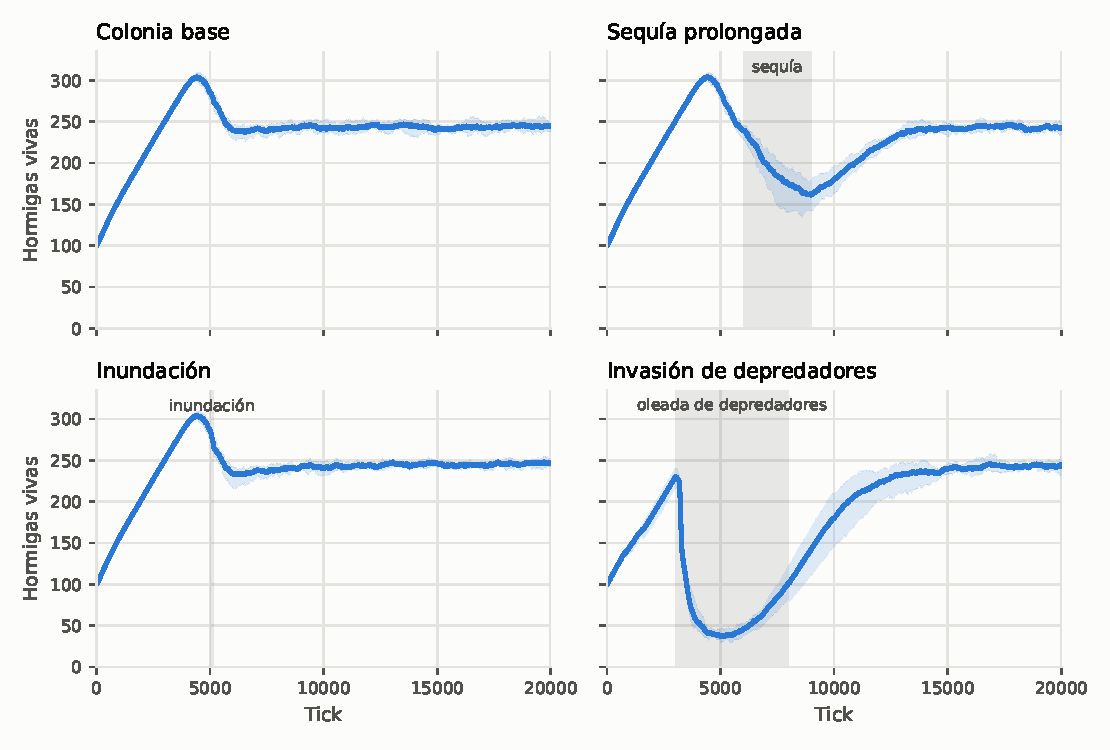
\includegraphics[width=\textwidth]{figuras/poblacion.pdf}
\caption{Población de hormigas por escenario. La línea es la media de cinco semillas y la banda va del mínimo al máximo; la zona gris marca el evento.}
\label{fig:poblacion}
\end{figure}

\paragraph{Colonia base.} La población crece desde 100 hasta un pico de 306 cerca del tick 4500 y se estabiliza en $244\pm 4$ (entre 238 y 248 según la semilla), entre 2,4 y 2,5 veces la inicial. La banda entre semillas es muy estrecha: el sistema es robusto frente al azar.

\paragraph{Sequía.} La población cae en promedio un 34\,\% respecto de su valor al inicio de la sequía (de 25 a 45\,\% según la semilla) y se recupera en las cinco semillas, entre 3900 y 5800 ticks después de terminar. La sequía actúa por dos caminos: baja la regeneración de la comida y encarece la energía de las hormigas fuera del nido, así que mueren más por hambre (131 por corrida, frente a 21 en la colonia base).

\paragraph{Inundación.} Mueren entre \muertesinundacionmin{} y \muertesinundacionmax{} hormigas por ahogamiento y la colonia sobrevive en las cinco semillas. En la tabla~\ref{tab:resumen} la recuperación aparece como 0/5, pero es un efecto de la métrica: la inundación empieza en el tick 5000, cuando la colonia todavía está en la bajada del pico (cerca de 285 hormigas), por encima del equilibrio de largo plazo (cerca de 245). La población vuelve a su equilibrio, pero no supera la cifra previa. Es una limitación de definir la recuperación como ``volver a la población previa''.

\paragraph{Invasión de depredadores.} La oleada de 30 depredadores reduce la población, en promedio, un 85\,\% (hasta 29--43 hormigas) y la colonia se recupera en las cinco semillas. Los depredadores causan el \comparteinvasion\,\% de las muertes (22 a 27\,\% por semilla); el resto es hambre (el miedo y la huida interrumpen el forrajeo) y vejez.

\subsection{Causas de muerte}

\begin{table}[H]
\centering
\caption{Muertes acumuladas por causa en 20\,000 ticks (media de cinco semillas).}
\label{tab:muertes}
\begin{tabular}{@{}lrrrr@{}}
\toprule
\textbf{Escenario} & \textbf{Vejez} & \textbf{Hambre} & \textbf{Depredadores} & \textbf{Inundación} \\
\midrule
\tablamuertes
\bottomrule
\end{tabular}
\end{table}

\begin{figure}[tbp]
\centering
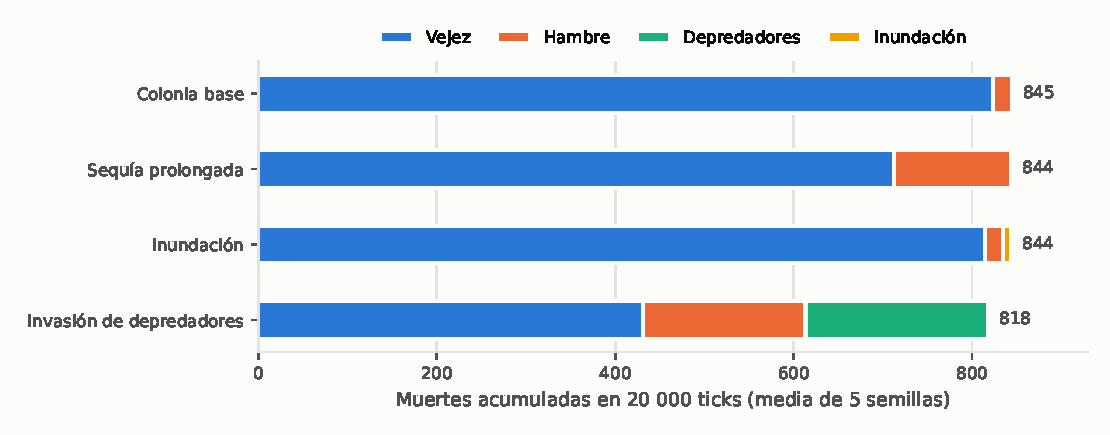
\includegraphics[width=\textwidth]{figuras/muertes.pdf}
\caption{Composición de las muertes por escenario. La longitud total es parecida en los cuatro: la colonia reemplaza lo que pierde, pero cambia de dónde vienen las pérdidas.}
\label{fig:muertes}
\end{figure}

\subsection{Verificación contra equilibrios analíticos}

El modelo SD tiene equilibrios que se pueden calcular a mano, y sirven para comprobar la implementación. Con comida abundante, la puesta es $P \approx p_{\max}=0{,}05$ huevos por tick. Entonces:

\begin{itemize}
  \item Huevos en equilibrio: $E^* = P\,\tau_e = 0{,}05\times200 = 10$.
  \item Larvas en equilibrio: $L^* = P\,\tau_l = 0{,}05\times400 = 20$.
  \item Obreras: el flujo de nacimientos es $P$ y la vida media es de 5000 ticks, así que $W^* \approx 0{,}05\times5000 = 250$.
\end{itemize}

La figura~\ref{fig:nidosim} muestra que los huevos y las larvas convergen a 10 y 20, y la población media final es de 244, a un 2\,\% del valor teórico. El pico de 306 cerca del tick 4500 no contradice el equilibrio y es consistente con la muerte de la cohorte inicial: las 100 hormigas iniciales se crean con edad cero y tienen una esperanza de vida cercana a 5000 ticks. No verificamos esta explicación con un experimento aparte.

\begin{figure}[tbp]
\centering
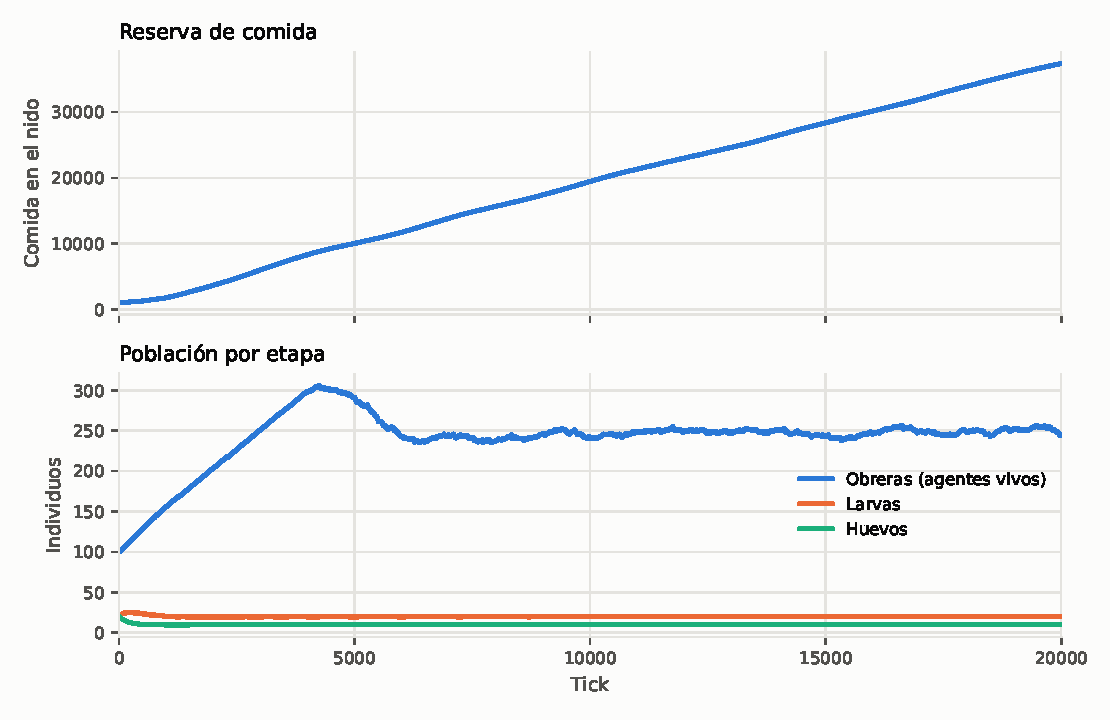
\includegraphics[width=\textwidth]{figuras/nido.pdf}
\caption{Stocks del nido en la colonia base (semilla 1). Arriba, la reserva de comida; abajo, obreras, larvas y huevos. Huevos y larvas convergen a los equilibrios analíticos 10 y 20.}
\label{fig:nidosim}
\end{figure}

\subsection{El proceso iterativo: qué cambió con las correcciones}

La tabla~\ref{tab:ablacion} compara tres versiones con las mismas semillas. La primera usa la misma configuración calibrada pero el comportamiento de \code{Colony} anterior a las correcciones del forrajeo. La segunda usa el código final con los parámetros por defecto del esquema. La tercera es la versión final.

\begin{table}[H]
\centering
\caption{Colonia base con cinco semillas y 20\,000 ticks, según la versión del código y la configuración.}
\label{tab:ablacion}
\begin{tabularx}{\textwidth}{@{}Xrrrr@{}}
\toprule
\textbf{Versión} & \textbf{Vivas} & \textbf{Colapso (ticks)} & \textbf{Pico medio} & \textbf{Comida entregada} \\
\midrule
Forrajeo anterior, configuración calibrada & 0/5 & 2877--11\,452 & 130 & 1131 \\
Código final, parámetros por defecto & 0/5 & 753--840 & 108 & 22 \\
Código final, configuración calibrada & 5/5 & -- & 306 & 45\,472 \\
\bottomrule
\end{tabularx}
\end{table}

Dos conclusiones. Primero, las correcciones del forrajeo son necesarias: sin ellas, la misma configuración entrega cuarenta veces menos comida y la colonia se extingue. Segundo, los parámetros por defecto del esquema no son viables (regeneración de comida de cero y consumo alto); esto es una limitación conocida y la tratamos en la sección~\ref{sec:conclusion}.

Los defectos del forrajeo que se corrigieron, y cómo se detectó cada uno, fueron: las hormigas con carga seguían el máximo local de feromona de hogar y se alejaban del nido; las buscadoras se alejaban sin límite en caminatas casi rectas; al huir con carga, las hormigas la perdían al recoger de nuevo; recogían migajas de 0,02 unidades; y, cuando ya no quedaban depredadores, las hormigas en huida no volvían nunca a su estado normal. Además, con velocidades de 2 celdas por tick, el radio de captura fijo de 1 celda hacía que los depredadores sobrepasaran a su presa y casi no cazaran, por lo que el radio ahora escala con la velocidad.

\subsection{Calidad técnica}

\begin{table}[H]
\centering
\caption{Verificaciones técnicas.}
\label{tab:calidad}
\begin{tabularx}{\textwidth}{@{}Xl@{}}
\toprule
\textbf{Verificación} & \textbf{Resultado} \\
\midrule
Pruebas del backend (pytest) & 136 pasan \\
Pruebas del frontend (Vitest) & 66 pasan \\
Compilación del frontend y tipos desde el contrato & Sin errores ni cambios \\
Determinismo (misma semilla, 500 ticks, con obstáculo, comida y sequía) & Cuadros idénticos \\
Invariante $W$ = hormigas vivas, 2000 ticks & Se cumple en cada tick \\
Mínimo del resumen exacto con el historial compactado & Se cumple \\
Tiempo de un tick (2000 hormigas, 50 depredadores, $200\times200$) & \msportick\,ms (límite 15\,ms) \\
\bottomrule
\end{tabularx}
\end{table}

\subsection{Criterios de calibración}

\begin{table}[H]
\centering
\caption{Criterios acordados para los escenarios (semillas 1 a 5, 20\,000 ticks) y resultado.}
\label{tab:criterios}
\begin{tabularx}{\textwidth}{@{}lXXl@{}}
\toprule
\textbf{Escenario} & \textbf{Criterio} & \textbf{Observado} & \textbf{Cumple} \\
\midrule
Base & Sobrevive; final entre 1,2 y 5 veces la inicial & 5/5 vivas; 2,4 a 2,5 veces & Sí \\
Sequía & Caída $\geq15\,\%$; recuperación en $\geq3$ de 5 & Caída de 25 a 45\,\%; 5/5 & Sí \\
Inundación & Muertes por inundación $>0$; sobrevive & 6 a 17 muertes; 5/5 vivas & Sí \\
Invasión & Depredadores $>20\,\%$ de las muertes; sobrevive en $\geq3$ de 5 & \comparteinvasion\,\%; 5/5 vivas & Sí \\
\bottomrule
\end{tabularx}
\end{table}

% ---------------------------------------------------------------------------
\section{Conclusión}\label{sec:conclusion}

Construimos un modelo híbrido en el que los agentes y el nido se retroalimentan: lo que entregan las hormigas alimenta la puesta, la maduración repone a los agentes y el tamaño y el hambre de la colonia cambian su estrategia de forrajeo. El acoplamiento respeta sus invariantes en cada tick y sus equilibrios coinciden con el cálculo analítico (huevos 10, larvas 20 y 244 obreras frente a 250). Con cinco semillas, la colonia sobrevive a una sequía, una inundación y una invasión, y cada perturbación deja una huella distinta en las causas de muerte, como el planteamiento original esperaba.

Hallazgos principales:
\begin{enumerate}
  \item El equilibrio de población de la colonia calibrada lo fija la demografía (puesta $\times$ esperanza de vida), no la comida: la reserva del nido crece sin límite (figura~\ref{fig:nidosim}).
  \item En nuestros experimentos, la sequía afecta a la colonia sobre todo porque encarece la energía de las hormigas fuera del nido; la baja regeneración de comida pesa menos porque la reserva del nido amortigua.
  \item La invasión de depredadores mata menos por captura directa que por interrupción del forrajeo: el hambre es casi tan importante como los depredadores.
  \item La eficacia del forrajeo dependía de detalles de movimiento fáciles de pasar por alto. Sin las correcciones, la misma configuración entrega cuarenta veces menos comida.
\end{enumerate}

\subsection{Limitaciones}

\begin{itemize}
  \item \textbf{Parámetros por defecto no viables.} Con la regeneración de comida en cero, la colonia colapsa en unos 800 ticks. Los escenarios usan una configuración calibrada. No cambiamos los valores por defecto porque forman parte del contrato de la API.
  \item \textbf{Reserva del nido sin tope.} La comida almacenada crece sin límite, lo que amortigua las sequías. Un tope de almacenamiento o una regulación del forrajeo según la reserva sería más realista.
  \item \textbf{Régimen limitado por comida inestable.} Cuando subimos el consumo hasta que la comida sí limitaba a la colonia, el sistema oscilaba y varias semillas se extinguían. El modelo estable es el que se limita por demografía.
  \item \textbf{Dependencia de la semilla.} Las fuentes de comida se colocan al azar; en semillas con fuentes lejanas el forrajeo es difícil. Añadimos fuentes para dar robustez, pero la sensibilidad persiste.
  \item \textbf{Calibración.} Los parámetros se ajustaron con las semillas 1 a 5 y no se validaron con semillas nuevas ni con datos empíricos.
  \item \textbf{Métrica de recuperación.} Definirla como ``volver a la población previa'' depende del momento del evento (caso de la inundación).
  \item \textbf{Verificación manual de la interfaz} pendiente de documentar: la revisión visual del frontend y las capturas para el video.
\end{itemize}

\subsection{Trabajo futuro}

Colonias rivales (como en los modelos de referencia con energía), feromonas repelentes, tope de almacenamiento, comparación con datos de campo, un análisis de sensibilidad de parámetros y validación con semillas no usadas en la calibración.

% ---------------------------------------------------------------------------
\bibliographystyle{plain}
\nocite{*}
\bibliography{referencias}

\end{document}
